

All input values required to plot Fig. \ref{constr/52/tab:table1} are given in Table \ref{constr/52/tab:table1} as shown below

\begin{table}[!ht]
\begin{center}
    \resizebox{\columnwidth}{!}{
\begin{tabular}{ | m{2cm} | m{1.5cm}| m{2cm} | m{1.5cm} |} 
\hline
& Symbols & Circle1 & Circle2 \\
\hline
Centre & $\vec{O}$ & \myvec{0\\0} & \myvec{0\\0} \\ 
\hline
Radius & $r_{1}$,$r_{2}$ & 2.5 & 4 \\ 
\hline
Polar coordinate & $\vec{C}_{1}$,$\vec{C}_{2}$ & 2.5\myvec{\cos \theta\\  \sin \theta} & 4\myvec{\cos \theta\\  \sin \theta} \\
\hline
Angle & $\theta$ & 0-2$\pi$ & 0-2$\pi$ \\
\hline
\end{tabular}
    }
\end{center}
\caption{Input values}
\label{constr/52/tab:table1}
\end{table}


\begin{figure}[!ht]
\centering
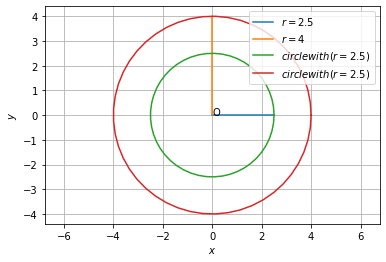
\includegraphics[width=\columnwidth]{solutions/52/Figure3.png}
\caption{Concentric circles with centre as origin and radii 2.5 and 4 respectively}
\label{constr/52/fig:circle}	
\end{figure}


